
\chapter{Feed Forward Neural Network in C++ 17 and OpenMP for performance optimization}

\section{Abstract}


In the project for course ECE 572, I will implement a feed forward neural network with sigmoid activation function. 

\section{Introduction}

Artificial Neural Networks (ANNs) are used in wide range of applications including system modeling and identification, signal processing, image processing, control systems and time series forecasting. The baseline of those models is a special class called Feed Forward Neural Network\cite{bebis1994nns,murat2006overview}. In this subclass of models, data is propagated forward only, and the model parameters are grouped in layers with no intra-communication. There is theoretically an infinite number of possible architecture regarding this type of models, hence they can have a lot of layers. In fact, Feed Forward Neural Networks were the beginning of a new Artificial Intelligence (AI) sub-field called Deep Learning, where the models used are designed to capture complicated patters. For that purpose, the model architecture as well as the dataset used to train them is very large. Consequently, in such cases the model performance poses a substantial challenge. There are several attempts on efficient ANN implementation using techniques, such as parallelization, to exploit the computational capabilities of the system architecture running a model\cite{huqqani2013multicore}. Using low-level programming languages, such as C++\cite{stourstrup2013cpp}, and frameworks that enable advanced parallelization and efficient data handling techniques, such as OpenMP\cite{dagum1998openmp}, the programmer can achieve better results in terms of performance compared to most state-of-the-art Deep Learning frameworks\cite{Jang2008NeuralNI}. 

\par

For the project of course ECE 572, I will try to implement a feed forward model with sigmoid activation function. The user will have to make little to no configurations before the execution of the driver. It will be fully re-configurable regarding the architecture of the model. For example, the user will be able to define the layers and number of neurons using command line arguments. Moreover, the software architecture will follow that of well known deep learning frameworks, such as PyTorch\cite{paszke2019pytorch}. That way the user will be able to easily navigate around the project if there is some prior experience with such frameworks. Furthermore, the user will be kept well informed throughout the data loading, the training and the inference process with \textit{progress bars}. Finally, the advantages of the proposed project will be demonstrated using a well known dataset, Fashion MNIST\cite{FashionMNIST2017Xiao}.

\section{Challenges}

The implementation of a neural network in theory is an easy process. However, when it comes to putting together those formulas using software, the engineer is challenged to compile an efficient code implementation. The challenge becomes even greater when the project is carried out in a low-level programming language, such as C++, where the engineer has to solve substantial numerical and challenges since the project is based on scientific computation. After solving those challenges, the engineer has to structure the code in order to implement parallel software architectures and data pipelining for efficient execution. In this project, the optimization part will utilize the OpenMP framework for software parallelization and extreme device utilization.

\section{Comparison}

To actually realize the magnitude of optimization achieved by the parallel version of the project, I've implemented $2$ more versions. The first is the \textit{Python} version using \textit{PyTorch}, which is the fastest deep learning framework in Python. The second is a \texttt{C++} implementation of the proposed feed forward neural network model running in serial mode. The \textit{Python} version was implemented to capture the performance gap compared to the \texttt{C++} implementation. The results after training using the \textit{Python} implementation can be viewed at figure \ref{fig:python}. The results after training using the \texttt{C++} serial implementation can be viewed at figure \ref{fig:cpp-serial}. It is already clear that the \texttt{C++} implementation of the Feed Forward Neural Network is dominant. In fact the performance boost is above $1,000 \; \%$.

\begin{figure}[!htbp]
\centering
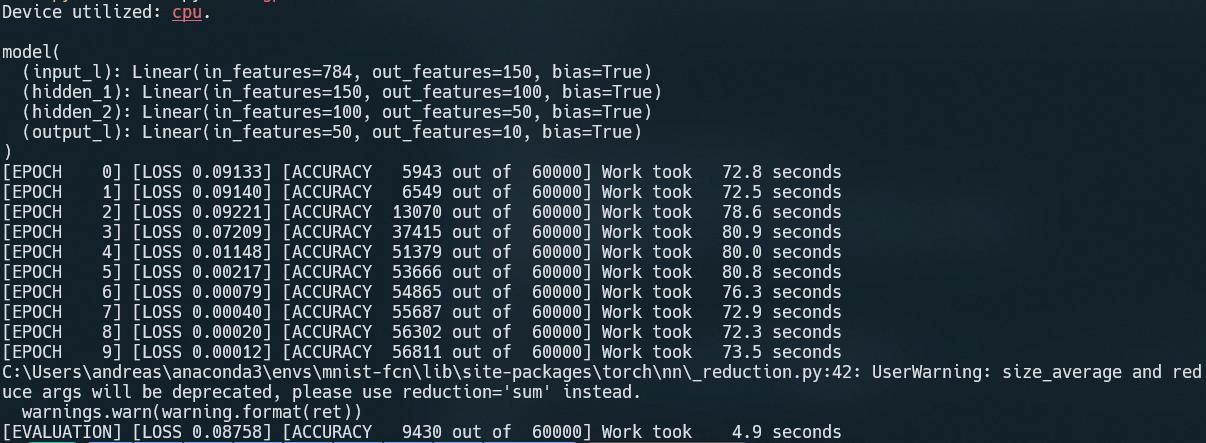
\includegraphics[width=\linewidth]{static/figures/python.PNG}
\caption{Results from the Python implementation.}
\label{fig:python}
\end{figure}

\begin{figure}[!htbp]
\centering
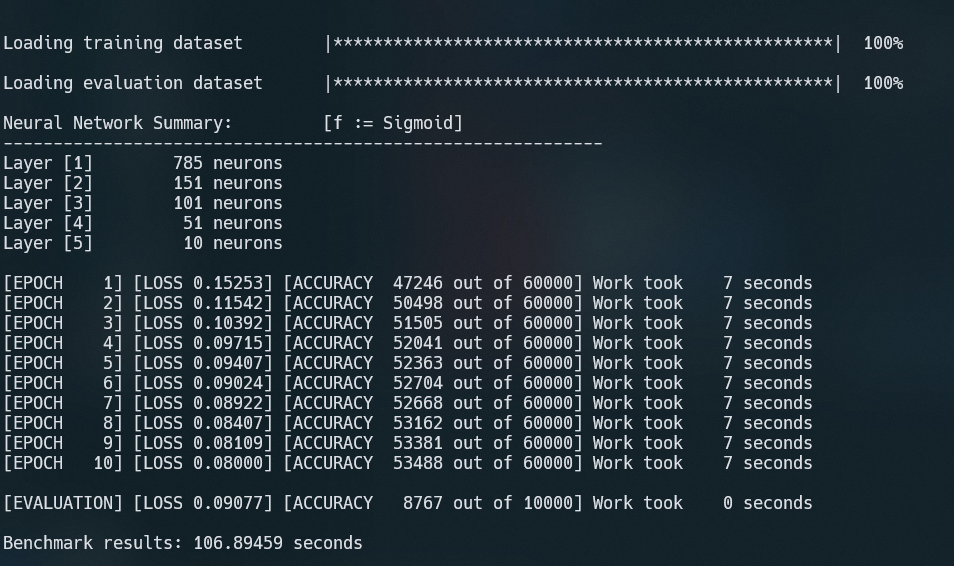
\includegraphics[width=\linewidth]{static/figures/cpp-serial.PNG}
\caption{Results from the serial \texttt{C++} implementation.}
\label{fig:cpp-serial}
\end{figure}

The code for those implementations can be found at \url{https://github.com/AndreasKaratzas/ece572}. The repository is currently private. If you would like to gain access please email at \href{mailto:andreas.karatzas@siu.edu}{andreas.karatzas@siu.edu} with your GitHub account, and I will add you as a collaborator.

\section{Parallel Implementation}

After having reviewed the benchmarks from the \textit{Python} version and the serial \texttt{C++} implementation, we are ready to proceed with the parallel \texttt{C++} implementation. The effective core utilization percentage can be reviewed in figure \ref{fig:cpp-parallel-vtune}.

\begin{figure}[!htbp]
\centering
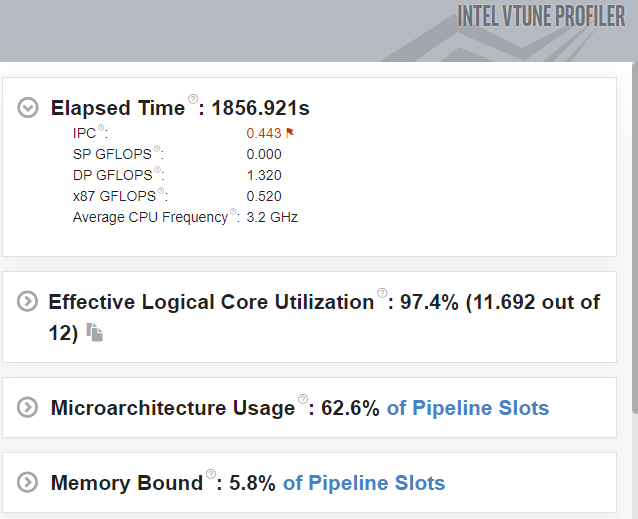
\includegraphics[width=\linewidth]{static/figures/vtune.PNG}
\caption{Effective Core Utilization using Intel VTUNE.}
\label{fig:cpp-parallel-vtune}
\end{figure}

Finally, in figure \ref{fig:cpp-parallel} we can review a sample execution of our project. It is clear that we achieved more than $200 \; \%$ performance boost.

\begin{figure}[!htbp]
\centering
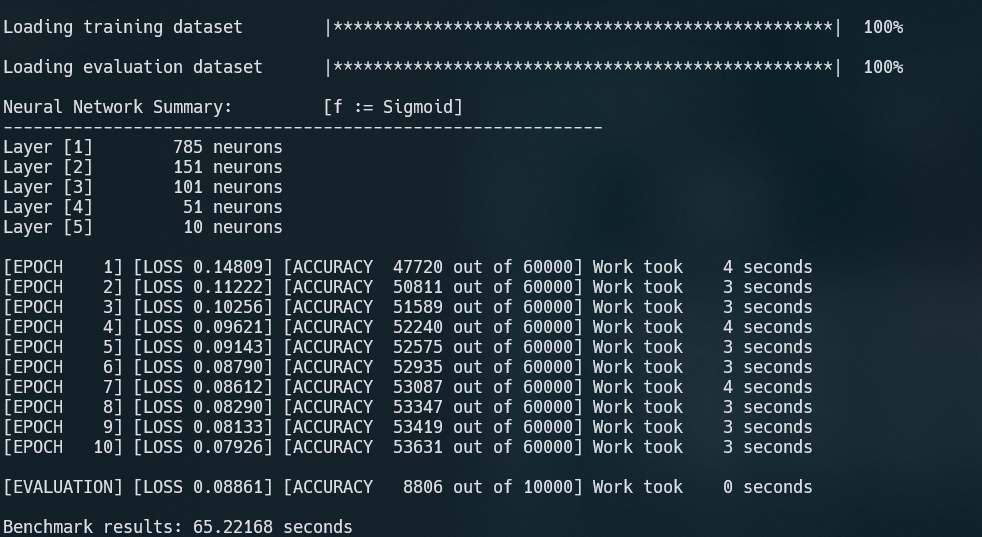
\includegraphics[width=\linewidth]{static/figures/cpp-parallel.PNG}
\caption{Results from the parallel \texttt{C++} implementation.}
\label{fig:cpp-parallel}
\end{figure}

Therefore, we can safely conclude that the project was a success since we gradually dropped the training time from $73$ seconds to down to just $3$ seconds per epoch.

\section{Important Project Classes}

The main project classes are:
\begin{itemize}
\item The \emph{dataset} class
\item The \emph{nn} class
\end{itemize}

\subsection{The dataset class}

The dataset class handles the data that is being fed to the neural network. It includes the following features:
\begin{itemize}
\item Initialization of the a dataset instance using a CSV file.
\item Print dataset.
\end{itemize}

A normalization process is also carried out during the data parsing phase. The normalization is based on a user defined value. This feature helps to reduce computational errors and achieve better results. If data is not properly normalized before training, then there is a good chance of neuron overflow, due to the sigmoid function. To initialize a dataset, the user must know the number of classes that exist in the dataset. THe user is required to also know the number of dataset samples. The type of data found in the dataset must be integers for the purpose of this project. Finally, the first column has to contain the class label of the corresponding sample, and the first row of the CSV must be a verbal description of the corresponding column.

\subsection{The nn class}
\label{nn}
The \emph{nn} class handles the neural network defined by the user. The user has the option to change the structure of the neural network. The user is asked to give the proper number of input and output neurons with respect to the number of input vector elements and the number of classes of the dataset that will be used to train the model. Moreover, the model structure is dynamic. In other words, the user can define custom number of hidden layers and neurons. The structure is defined by the user using command line arguments. There are 3 types of command line arguments that are used to shape a model:
\begin{itemize}
\item \verb|-i|: this argument corresponds to the number of input neurons. For example, \verb|-i 784| corresponds to 785 (784 + 1 bias) input neurons\footnote{The \emph{bias} is added automatically, and therefore is not needed to be defined by the user.}.
\item \verb|-h|: this argument defines the number of neurons in a hidden layer. The user has the option to create a lot of hidden layers. For example, \verb|-h 100 -h 50| tells the executable to create a model with $2$ hidden layers, the first will have 101 (100 + 1 bias) neurons, and the second 51 (50 + 1  bias) neurons.
\item \verb|-o|: this argument corresponds to the number of output neurons. For example, \verb|-o 10| corresponds to an output layer of 10 neurons. Let it be noted that there is no bias neuron in the output layer.
\end{itemize}

All neurons utilize the sigmoid function to determine active state. The aforementioned arguments must be given in that same order to the executable. An example model defined for the purpose of this project would be:
\begin{itemize}
\item For a Windows OS system: \verb|.\nn.exe -i 784 -h 100 -o 10|
\item For a UNIX system: \verb|.nn -i 784 -h 100 -o 10|
\end{itemize}

Another useful hyper-parameter is the learning rate of the neural network. That rate is also defined at \verb|Common.hpp| header and defaults to $0.1$. This feature helps the model to avoid falling into some kind of local minima.

\section{Implementation Analysis}

In this paragraph, we go through analyzing the code for this project. To install the project, there instructions in paragraph \ref{git}. To better understand the software architecture, we will describe the key-points of this project:
\begin{itemize}
\item The synapses of each layer are saved in the \verb|weights| variable that lives in the \verb|nn| class.
\item The state of every neuron, i.e. the sum accumulated from neurons in the previous layer, are saved in the \verb|z| variable that lives in the \verb|nn| class.
\item The result for each neuron after its activation is saved in the \verb|a| variable that lives in the \verb|nn| class.
\item The \verb|forward| routine that is defined at \verb|nn| class implements forward propagation.
\item The \verb|back_propagation| routine computes the error for each neuron, whereas the \verb|optimize| routine backward-propagates each neuron's error. Both of those routines are defined at the \verb|nn| class.
\end{itemize}

\subsection{Driver.hpp and Driver.cpp}

These files are the driver files responsible for the project execution. In the header file, we define the auxiliary header files. Those extra header files will be used throughout the project for various tasks.

\subsection{neural.hpp}

In the \verb|neural.hpp| header file, we have defined the neural network class. The object of this class are instances of type \verb|nn|. Every function of this header file is defined at:
\begin{itemize}
\item \verb|fit.cpp|. In this file, we define the functions responsible for model training and evaluation.
\item \verb|forward.cpp|. In this file, we define the forward propagation algorithm.
\item \verb|optimize.cpp|. In this file, we define the backwards propagation algorithm and optimization process.
\item \verb|loss.cpp|. In this file, we define the error function (criterion) used for error computation.
\item \verb|utilities.cpp|. In this file, we define functions used to initialize the model parameters. We also define a function called \verb|zero_grad|, which resets the state of the training algorithm before each epoch, in order to avoid processing garbage data. There is also a function named \verb|predict| which calls the neural network using user-defined data. However, the user is responsible for the normalization of that data. Finally, we have implemented \verb|summary| function that prints the neural network structure after compilation.
\item \verb|accuracy.cpp|. In this file, we define the function that evaluates the model accuracy.
\item \verb|export.cpp|. In this file, we define a function that exports all model parameters in order to be used at a later time for inference.
\end{itemize}

\subsection{activation.hpp and activation.cpp}

In these files, we have created some modules that are used for neuron activation. There are 2 implementation of the sigmoid function. For better precision, we utilized the \verb|std::pow()| function of the \verb|math.h| (or \verb|cmath|) library. We also tested the \verb|std::exp()| function of the same library. However, due to numerical issues, this function returned inaccurate or sometimes false results. That motivated us to create a custom implementation of the aforementioned function using Taylor series approximation. We also implemented the \textit{ReLU} activation function. In the code however, we solo-utilized the safe version of sigmoid function.

\subsection{interface.hpp and interface.cpp}

In these files, we have defined functions that implement a basic GUI. The GUI is responsible to keep the user informed on:
\begin{itemize}
\item The epoch error and accuracy.
\item The epoch expected latency.
\item Model summary.
\end{itemize}

There are a lot of extra function implemented, but they are currently not cross-platform and therefore are not utilized for the purpose of this project\footnote{Let this be considered as future work.}.

\subsection{parser.hpp and parser.cpp}

In these files, we define functions that help in the command line argument parsing process. There are some safety-check routines implemented in case the user doesn't use the command line arguments in a proper way. However, there are not that extensive and therefore the user is remind to use the command line arguments with caution as described at \ref{nn}.

\subsection{common.hpp}

In this header file, we have defined all program hyper-parameters, such as the number of epochs and the learning rate (\verb|EPOCHS| and \verb|LEARNING_RATE|). We also define a \textit{filepath} for the validation subset. Moreover, we also define the number of training samples and the number of classes found in the dataset. Finally, we also define the number of threads used to make the most of project run in a parallel fashion. We recommend the number of threads to be equal to the number of logical cores found in the system.
